	\tikzset{every picture/.style={line width=0.75pt}} %set default line width to 0.75pt        
	
	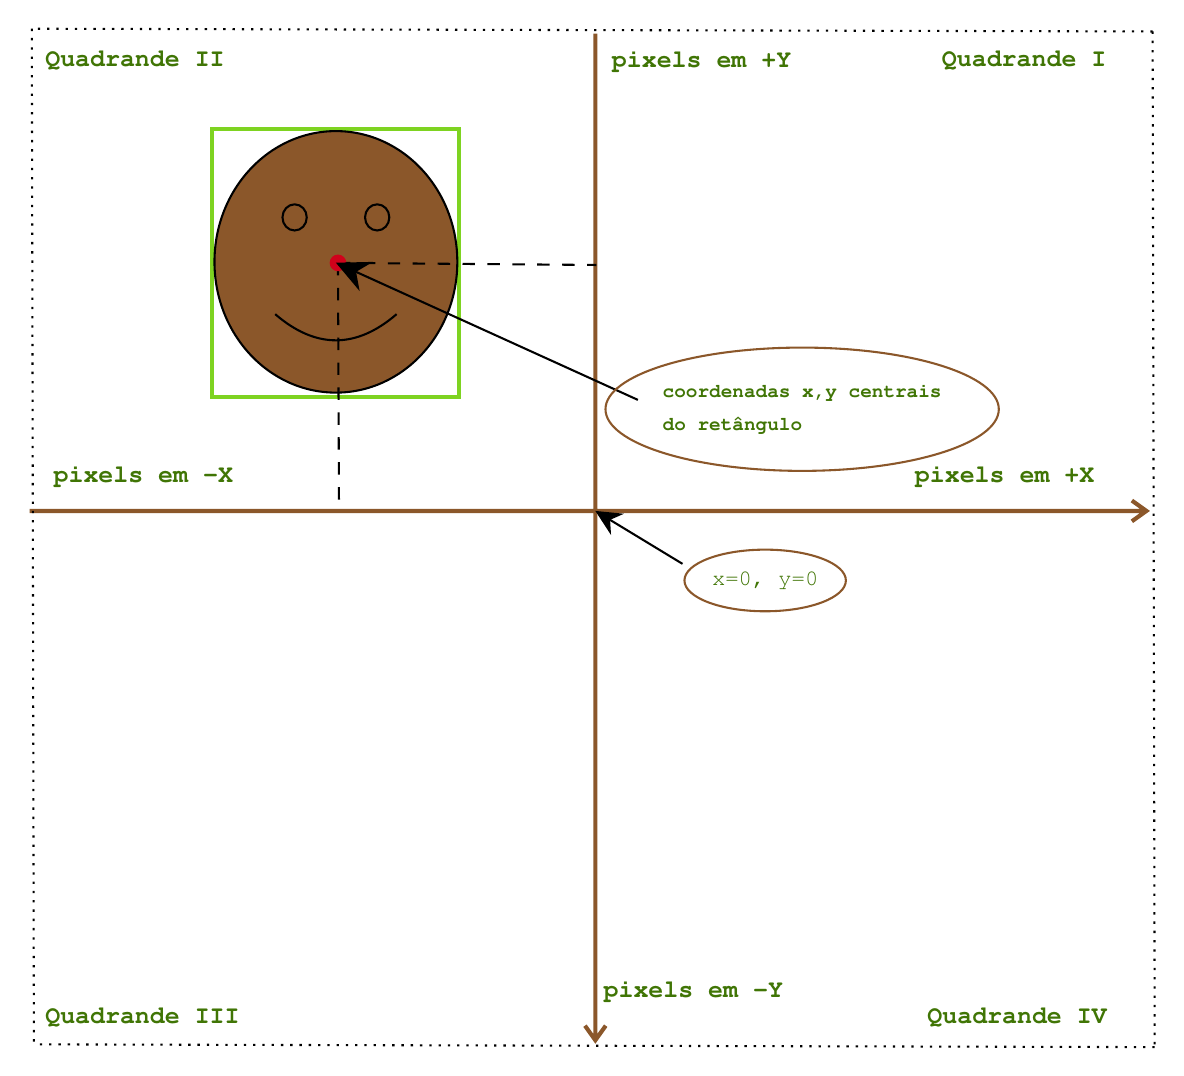
\begin{tikzpicture}[x=0.75pt,y=0.75pt,yscale=-1,xscale=1]
	%uncomment if require: \path (0,578); %set diagram left start at 0, and has height of 578
	
	%Shape: Axis 2D [id:dp745366717574464] 
	\draw [color={rgb, 255:red, 139; green, 87; blue, 42 }  ,draw opacity=1 ][line width=1.5]  (281.5,12) -- (281.5,497)(547,242) -- (9,242) (286.5,490) -- (281.5,497) -- (276.5,490) (540,237) -- (547,242) -- (540,247)  ;
	%Shape: Rectangle [id:dp835814910936395] 
	\draw  [color={rgb, 255:red, 126; green, 211; blue, 33 }  ,draw opacity=1 ][line width=1.5]  (97,187) -- (97,57.8) -- (216,57.8) -- (216,187) -- cycle ;
	%Shape: Smiley Face [id:dp00370584545415098] 
	\draw  [fill={rgb, 255:red, 139; green, 87; blue, 42 }  ,fill opacity=1 ] (98,122) .. controls (98,87.21) and (124.19,59) .. (156.5,59) .. controls (188.81,59) and (215,87.21) .. (215,122) .. controls (215,156.79) and (188.81,185) .. (156.5,185) .. controls (124.19,185) and (98,156.79) .. (98,122) -- cycle ; \draw  [fill={rgb, 255:red, 139; green, 87; blue, 42 }  ,fill opacity=1 ] (130.76,100.58) .. controls (130.76,97.1) and (133.38,94.28) .. (136.61,94.28) .. controls (139.84,94.28) and (142.46,97.1) .. (142.46,100.58) .. controls (142.46,104.06) and (139.84,106.88) .. (136.61,106.88) .. controls (133.38,106.88) and (130.76,104.06) .. (130.76,100.58) -- cycle ; \draw  [fill={rgb, 255:red, 139; green, 87; blue, 42 }  ,fill opacity=1 ] (170.54,100.58) .. controls (170.54,97.1) and (173.16,94.28) .. (176.39,94.28) .. controls (179.62,94.28) and (182.24,97.1) .. (182.24,100.58) .. controls (182.24,104.06) and (179.62,106.88) .. (176.39,106.88) .. controls (173.16,106.88) and (170.54,104.06) .. (170.54,100.58) -- cycle ; \draw   (127.25,147.2) .. controls (146.75,164) and (166.25,164) .. (185.75,147.2) ;
	%Straight Lines [id:da45515329684866135] 
	\draw [color={rgb, 255:red, 0; green, 0; blue, 0 }  ,draw opacity=1 ] [dash pattern={on 0.84pt off 2.51pt}]  (550,11) -- (551,500.33) ;
	%Straight Lines [id:da24415373962833065] 
	\draw [color={rgb, 255:red, 0; green, 0; blue, 0 }  ,draw opacity=1 ] [dash pattern={on 0.84pt off 2.51pt}]  (551,500.33) -- (11,499) ;
	%Straight Lines [id:da6205263233417599] 
	\draw  [dash pattern={on 4.5pt off 4.5pt}]  (157.5,122.5) -- (282,123.5) ;
	%Straight Lines [id:da2467412144940746] 
	\draw  [dash pattern={on 4.5pt off 4.5pt}]  (157.5,122.5) -- (158,241.5) ;
	%Shape: Circle [id:dp6195483350711979] 
	\draw  [color={rgb, 255:red, 208; green, 2; blue, 27 }  ,draw opacity=1 ][fill={rgb, 255:red, 208; green, 2; blue, 27 }  ,fill opacity=1 ] (154,122.5) .. controls (154,120.57) and (155.57,119) .. (157.5,119) .. controls (159.43,119) and (161,120.57) .. (161,122.5) .. controls (161,124.43) and (159.43,126) .. (157.5,126) .. controls (155.57,126) and (154,124.43) .. (154,122.5) -- cycle ;
	%Straight Lines [id:da3852329060686428] 
	\draw    (302,188.5) -- (159.23,123.64) ;
	\draw [shift={(156.5,122.4)}, rotate = 384.43] [fill={rgb, 255:red, 0; green, 0; blue, 0 }  ][line width=0.08]  [draw opacity=0] (16.07,-7.72) -- (0,0) -- (16.07,7.72) -- (10.67,0) -- cycle    ;
	%Straight Lines [id:da7942156802276659] 
	\draw    (323.5,267.5) -- (284.06,243.56) ;
	\draw [shift={(281.5,242)}, rotate = 391.26] [fill={rgb, 255:red, 0; green, 0; blue, 0 }  ][line width=0.08]  [draw opacity=0] (12.5,-6.01) -- (0,0) -- (12.5,6.01) -- (8.3,0) -- cycle    ;
	%Straight Lines [id:da8593503836199177] 
	\draw [color={rgb, 255:red, 0; green, 0; blue, 0 }  ,draw opacity=1 ] [dash pattern={on 0.84pt off 2.51pt}]  (10,9.67) -- (11,499) ;
	%Straight Lines [id:da5989886602637362] 
	\draw [color={rgb, 255:red, 0; green, 0; blue, 0 }  ,draw opacity=1 ] [dash pattern={on 0.84pt off 2.51pt}]  (550,11) -- (10,9.67) ;
	
	% Text Node
	\draw (434,219) node [anchor=north west][inner sep=0.75pt]   [align=left] {{\fontfamily{pcr}\selectfont {\small \textbf{\textcolor[rgb]{0.25,0.46,0.02}{pixels em +X}}}}};
	% Text Node
	\draw (284,467) node [anchor=north west][inner sep=0.75pt]   [align=left] {{\fontfamily{pcr}\selectfont {\small \textbf{\textcolor[rgb]{0.25,0.46,0.02}{pixels em -Y}}}}};
	% Text Node
	\draw  [color={rgb, 255:red, 139; green, 87; blue, 42 }  ,draw opacity=1 ]  (363.32, 275.5) circle [x radius= 38.89, y radius= 14.85]   ;
	\draw (363.32,275.5) node   [align=left] {{\fontfamily{pcr}\selectfont {\footnotesize \textcolor[rgb]{0.25,0.46,0.02}{x=0, y=0}}}};
	% Text Node
	\draw  [color={rgb, 255:red, 139; green, 87; blue, 42 }  ,draw opacity=1 ]  (381.14, 193) circle [x radius= 94.75, y radius= 29.7]   ;
	\draw (381.14,193) node   [align=left] {{\fontfamily{pcr}\selectfont {\scriptsize \textbf{\textcolor[rgb]{0.25,0.46,0.02}{coordenadas x,y centrais}}}}\\{\fontfamily{pcr}\selectfont {\scriptsize \textbf{\textcolor[rgb]{0.25,0.46,0.02}{ do retângulo}}}}};
	% Text Node
	
	\draw (447,19) node [anchor=north west][inner sep=0.75pt]   [align=left] {{\fontfamily{pcr}\selectfont {\small \textbf{\textcolor[rgb]{0.25,0.46,0.02}{Quadrande I}}}}};
	
	\draw (15,19) node [anchor=north west][inner sep=0.75pt]   [align=left] {{\fontfamily{pcr}\selectfont {\small \textbf{\textcolor[rgb]{0.25,0.46,0.02}{Quadrande II}}}}};
	
	\draw (15,480) node [anchor=north west][inner sep=0.75pt]   [align=left] {{\fontfamily{pcr}\selectfont {\small \textbf{\textcolor[rgb]{0.25,0.46,0.02}{Quadrande III}}}}};
	
	\draw (440,480) node [anchor=north west][inner sep=0.75pt]   [align=left] {{\fontfamily{pcr}\selectfont {\small \textbf{\textcolor[rgb]{0.25,0.46,0.02}{Quadrande IV}}}}};
	
	\draw (288,19) node [anchor=north west][inner sep=0.75pt]   [align=left] {{\fontfamily{pcr}\selectfont {\small \textbf{\textcolor[rgb]{0.25,0.46,0.02}{pixels em +Y}}}}};
	% Text Node
	\draw (19,219) node [anchor=north west][inner sep=0.75pt]   [align=left] {{\fontfamily{pcr}\selectfont {\small \textbf{\textcolor[rgb]{0.25,0.46,0.02}{pixels em -X}}}}};
	
	
	\end{tikzpicture}
